
\documentclass[11pt,a4paper]{article}
\usepackage[hyperref]{AACL-IJCNLP2020}
\usepackage{times}
\usepackage{latexsym}
\renewcommand{\UrlFont}{\ttfamily\small}

\usepackage{microtype}


\newcommand\BibTeX{B\textsc{ib}\TeX}

\title{He Can Talk! Oh My Word, He can Talk!}

\author{First Author \\
  Affiliation / Address line 1 \\
  Affiliation / Address line 2 \\
  Affiliation / Address line 3 \\
  \texttt{email@domain} \\\And
  Second Author \\
  Affiliation / Address line 1 \\
  Affiliation / Address line 2 \\
  Affiliation / Address line 3 \\
  \texttt{email@domain} \\}

\date{}

\begin{document}

\maketitle

\author{\\
  Aner BarOz, Viktoria Brykalova, Oleksii Bulygin, Ivan Didur,\\
Vasyl Koida, David Levy, Gadi Mosenzon, Mykita Oliinyk,\\ 
Vlad Shanin, Yaroslav Taranov, Joshua Reuben, Joshua Rubin,\\
\thanks{ Use footnote for providing further information about author (webpage, alternative address)---\emph{not} for acknowledging funding agencies.  Funding acknowledgements go at the end of the paper.}    
\texttt{\{david,gadi\}@kamicomputing.com} \\
}

\newcommand{\fix}{\marginpar{FIX}}
\newcommand{\new}{\marginpar{NEW}}

\begin{abstract}
Voice interactions with computers (e.g. voice assistants) currently suffer from a number of problems which prevent human quality, voice conversation.

These problems can be divided into:
\begin{enumerate} %%[i]
  \item Open domain conversation  
  \item Prosody understanding and generation that operates in real-time
  \item Computing resources efficient. 
\end{enumerate}

In this work we show how all of these problems can be addressed by creating an end-to-end voice in, voice out neural network. We show that appropriate learning can improve voice interactions and bring them closer to human levels. 

We demonstrate that by using large language, graph and voice models, a natural language interaction is achieved. 

[Ivan to add a sentence to explain what is new]
\end{abstract}

\section{Introduction}
Currently, neural generation techniques have powered many inspiring applications, e.g., poem generation (Yang et al., 2018), neural machine translation
(NMT) (Bahdanau et al., 2015) and chatbot (Zhao
et al., 2017). Conditional (also known as controllable) text generation is an important task of text
generation, aiming to generate realistic text that
carries a specific attribute (e.g., positive or negative
sentiment). 

A common solution is to encode the
condition into a vector representation and then integrate it with the text generation process (Kingma ...).

These existing neural models have achieved
encouraging results. However, when a new condition is added (e.g., a new topic for categorical
generation), they require a full retraining or finetuning. This process is both time-consuming and
computationally inefficient (Houlsby et al., 2019).

Both fine-tuning and retraining are not desirable
in real-world applications since the delivery (e.g.,
transmitting updated weights through the Internet)
and client-side re-deployment (e.g., distribute updated weights to users) of large-scale weights are
often difficult.

Inspired by the recent success of Variational
Auto-Encoder (VAE) (Kingma and Welling, 2014)
based post-hoc conditional image generation strategy (Engel et al., 2018), we provide a new perspective for flexible conditional text generation. 


\section{Preliminaries}
\subsection{General framework}

\section{Methology}
block diagram comes here..
%% 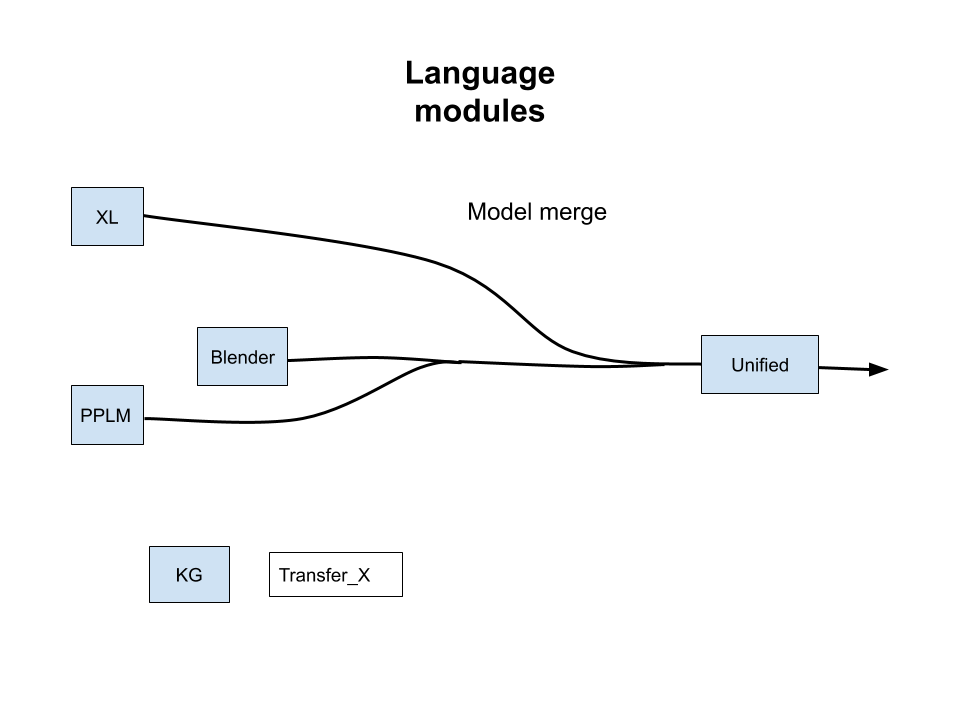
\includegraphics[width=0.8\textwidth,natwidth=610,natheight=642]{language_block_diagram.png}

\subsection{Language Understanding And Generation} %% thing related to language  
  
\subsubsection{Large Attention Language Model} %% Blender

\subsubsection{Autonomous Language Generation Control} % PPLM

\subsubsection{Knowledge Graph} % OpenDialKG



\subsection{Speech Modality}

\subsubsection{Inputs}
The baseline requirement from the user’s speech is for KAMI to know what the user
said. For this we employ Google’s 

<ORI> 

In addition to knowing what the user said, the system can benefit by knowing how the
user said it – what emotional state affected the user and caused the stress and intonation
that are evident in the speech data recognized by KAMI. 

Such emotion analysis on the
user’s voice characteristics is called “sentiment extraction”.


\subsubsection{Outputs}
The baseline requirement from KAMI’s speech is to convey the content of KAMI’s
responses, the spoken words, to the user. 

For this we employ the 
<WHATEVER – Ori to insert> 

text-to-speech system. 

In addition to conveying the words with which KAMI
is responding to the user, the system imposes on the spoken words an appropriate
prosody for conveying any required emphasis as well as KAMI’s emotional state.

\section{Experiments}
\subsubsection{Setup}

\subsubsection{Hyperparameters}

\subsubsection{Evaluation} % we use "pone"

\section{Results}

\section{Discussion}

\section{Related work}
<models papers here> 

\section{Conclusion}
In this paper, we present a novel speech generation framework for flexible conditional voice interaction. 
The extensive experiments demonstrate the superiority of the proposed framework against the existing alternatives on conditionality and diversity while allowing a new type of social oriented conversation.
Further more, we achievied new state of the art results. 

<actual numbers>

\section{Acknowledgments}
Thank yo Gadi for being what you are...

\section{References}


\begin{table}[t]
\caption{Sample table title}
\label{sample-table}
\begin{center}
\begin{tabular}{ll}
\multicolumn{1}{c}{\bf PART}  &\multicolumn{1}{c}{\bf DESCRIPTION}
\\ \hline \\
Dendrite         &Input terminal \\
Axon             &Output terminal \\
Soma             &Cell body (contains cell nucleus) \\
\end{tabular}
\end{center}
\end{table}



\bibliography{iclr2020_conference}
\bibliographystyle{iclr2020_conference}

\appendix
\section{Appendix}
You may include other additional sections here. 

\section{Credits}



\end{document}
